\documentclass[12pt]{beamer}
\usepackage{lmodern}
\usepackage{xcolor}
\usepackage{pgf,tikz}
%\usetikzlibrary{calc}
\usepackage{amssymb,amsmath,array,bm}
\usepackage[OT1,T2A]{fontenc}
\usepackage[utf8]{inputenc}
\usepackage[english,bulgarian]{babel}
\usepackage{hyperref}
\usepackage{multicol}
\usepackage{tabularx}


\def\fnmark#1{{\small}$^#1$}
\def\fnote#1#2{$^#1\;$\texttt{#2}\\}

\usepackage{verbatim}
%\usepackage[active,tightpage]{preview}
\usetheme{Madrid}

\usetikzlibrary{positioning,shapes,shadows,arrows}
\tikzstyle{myarrow}=[<-, >=open triangle 90, thick]
\tikzstyle{line}=[-, thick]

\begin{document}
	
	\date[УчИБАН'17]{УчИБАН \\ 2017}
	%\institute[SHSM]{Sofia High School of Mathematics \\ Sofia, Bulgaria}
	\author[Алекс, Антоан]{
		\begin{table}[]
			\begin{tabular}{rl}
				\normalsize{Автори:\      } & \normalsize{Алекс Цветанов и Антоан Георгиев} \\
				\scriptsize{Ментор:     } & \scriptsize{Доц. д-р Златогор Минчев}
			\end{tabular}
		\end{table}
	}
	\title[Виртуален асистент]{Виртуален асистент}
	\begin{frame}
		\titlepage
 	\end{frame}
	\begin{frame}
		\frametitle{Въведение}
		\begin{block}{}
			Основната цел на нашия проект е създаването на „виртуален асистент“, чрез най-новите технологии и прилагайки най-добрите практики при организирането на обучения, така че да са интерактивни, интересни, полезни и възможно най-улеснени за учениците. Най-важната част от проекта ни е да стимулираме учениците, показвайки им, че предметите не са толкова трудни, колкото изглеждат. \\
			\vspace{2ex}
			Асистентът ще отговаря на въпросите на учениците по съответните уроци и ще им предоставя допълнителна информация по темите, от които се интересуват.
		\end{block}
 	\end{frame}
	\begin{frame}
		\frametitle{Защо е полезен?}
		\begin{block}{Полезен е ...}
			\begin{itemize}
				\item ако искате да се самообучавате
				\item за да се модернизира образованието
			\end{itemize}
		\end{block}
		\begin{block}{Позволява на младите хора ...}
			\begin{itemize}
				\item да се докоснат до най-новите технолгии, чрез преживяване
			\end{itemize}
		\end{block}
		\begin{block}{Асистентът може да ...}
			\begin{itemize}
				\item провокира интереса на младите хора към предметите
			\end{itemize}
		\end{block}
	\end{frame}
	\begin{frame}
		\frametitle{Архитетктура}
		%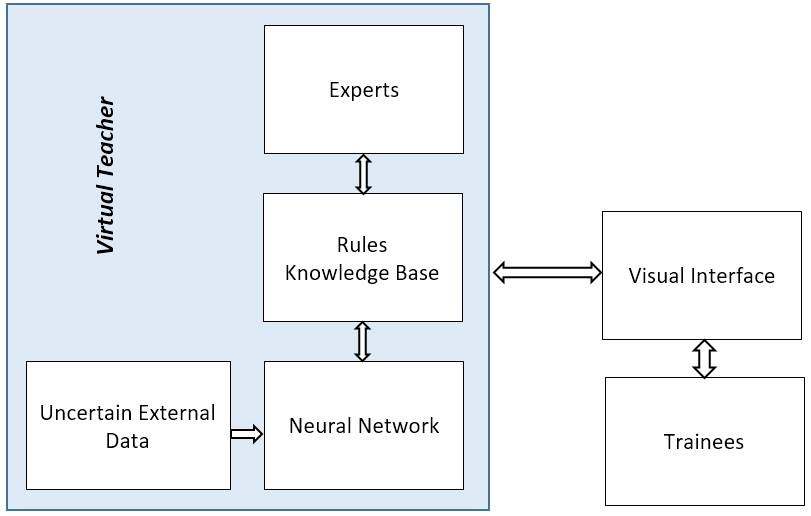
\includegraphics[width=\textwidth]{.../schema.jpg}
	\end{frame}
	\begin{frame}
		\frametitle{Иновации?}
		\begin{itemize}
			\item обединява 2 нови технологии - Изкуствен интелект \& Виртуална реалност
			\item Образованието става още по-близо до учениците
			\item Образованието става по-интерактивно
		\end{itemize}
	\end{frame}
	\begin{frame}
		\frametitle{Каква част от проекта е готова?}
		\begin{itemize}
			\item Трансформирането на прости изречения в мисловни карти
			\item Прототип на потребителския интерфейс
			АНТОАН ГЕОРГИЕВ ДА СЕ ЗАЕМЕ
		\end{itemize}
	\end{frame}
	\begin{frame}
		\frametitle{Какво следва?}
		\begin{itemize}
			\item Завършването на генератора на мисловни карти
			\item Изграждането на библиотеки за гласова и текстова комуникация с учениците
			\item Изграждането на VR приложение
			АНТОАН ГЕОРГИЕВ ДА СЕ ЗАЕМЕ
		\end{itemize}
	\end{frame}
	\begin{frame}
		\begin{center}
			{\Huge Демо на прототипа} \\ \vspace{1cm}
			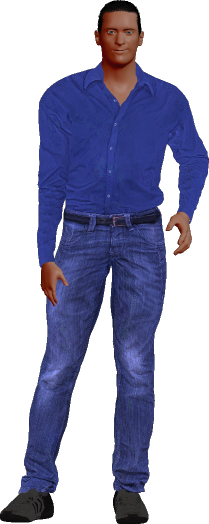
\includegraphics[scale=0.25]{../bad_boy.png}
		\end{center}
	\end{frame}
	\begin{frame}
		 	 	 Специални благодарности за:
		\begin{itemize}
			\item Златогор Минчев за изграждането на идеята
		\end{itemize}
		Благодарим също на:
		\begin{itemize}
			\item Ученически институт към БАН
			\item Българска академия на науките
			\item VR Express
			\item iGreet
		\end{itemize}
	\end{frame}
	
	\begin{frame}
	\frametitle{Ресурси}
		\begin{itemize}
			\item
			{\itshape Artificial Intelligence: A Modern Approach, \\ 3rd Edition, Prentice Hall, 2010}. \\
			\texttt{Stuart Russell \& Peter Norvig.} \\
			\item
			{\itshape Virtual\ objects\ seem\ totally\ real}.
			\\
			\item
			{\itshape Amelia}.
			\texttt{http://www.ipsoft.com/amelia/}. \\
			\item
			{\itshape The Future Of Chatbots And Artificial Intelligence}.
			\item
			{\itshape Your DNA Avatar - What Happens When Artificial Intelligence Meets Cutting-Edge Genetics?}.
			\item%{latex}
			{\itshape \LaTeX}.
			\texttt{https://www.latex-project.org/}.
		\end{itemize}
	\end{frame}
	
	\begin{frame}
	\begin{center}
	{\Huge Въпроси}\\
	
\includegraphics[scale=0.25]{../questions.png}
	\end{center}
	\end{frame}
	
	\begin{frame}
	\begin{center}
	{\Huge Благодарим\\за\\вниманието!}
	\end{center}
	\end{frame}

\end{document}
